Das Ergebnis des Hörversuchs ist in Abbildung ~\ref{fig:versuch} zu sehen. Es wurden insgesamt 5 Personen mit geschultem Gehör befragt.

\begin{figure}[!ht]
  \centering
  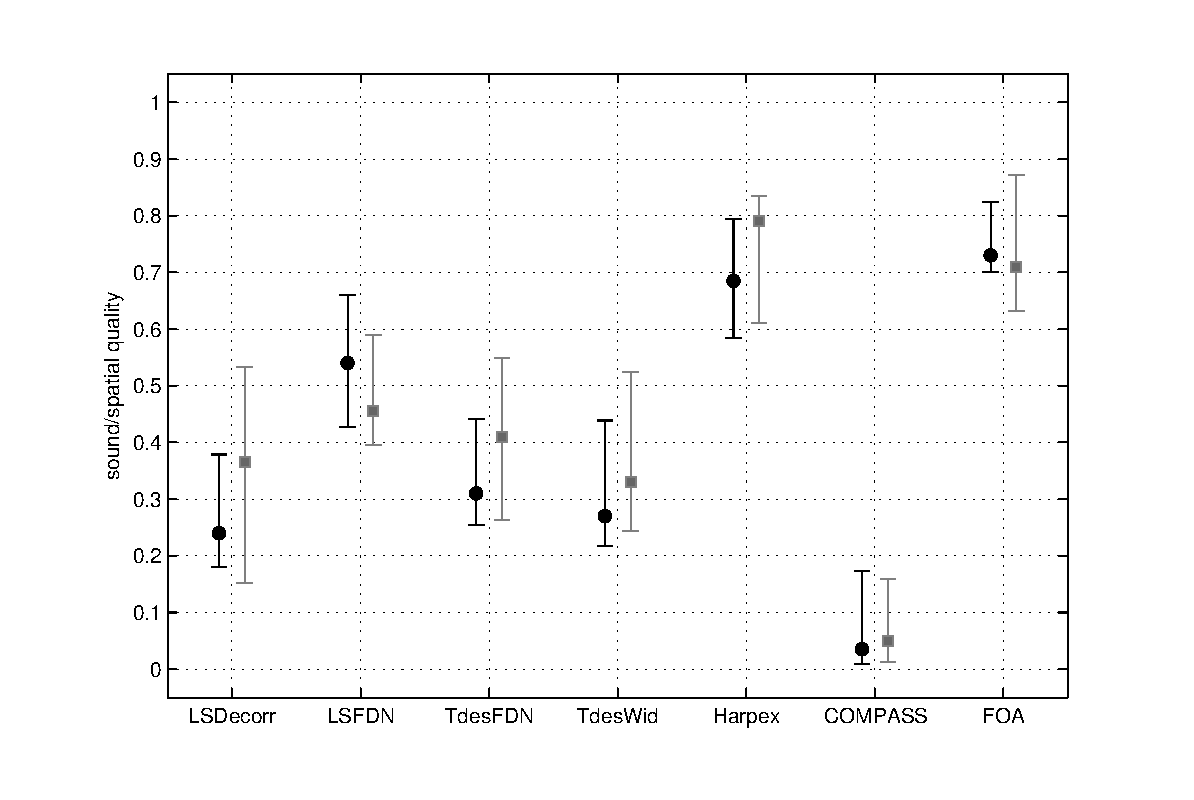
\includegraphics[width=0.9\textwidth]{ergebnis/plots/result.eps}
  \caption{Ergebnis des Hörversuchs, Median mit 95\% Konfidenzintervalle (Klangqualität in schwarz und räumliche Qualität in grau)}
  \label{fig:versuch}
\end{figure}

Die Bewertungen erfolgten nach zwei Kriterien:

\begin{itemize}
  \item Klangqualität: \textit{sehr gut} (1) bis \textit{sehr schlecht} (0)
  \item räumliche Qualität: \textit{realistisch} (1) bis \textit{synthetisch} (0).
\end{itemize}

Die Bewertungen nach den zwei gewählten Kriterien weisen eine teils hohe Korrelation auf (siehe Tab. \ref{tab:corr}). Dies deutet entweder auf eine tatsächliche Korrelation von Klangqualität und räumlicher Wiedergabequalität hin, oder die Fragestellung zielt nicht auf genügend unterschiedliche Aspekte der Testsignale ab. Dabei können stärkere Artefakte als Verminderung der räumlichen Qualität des Algorithmus gedeutet werden.

\begin{table}
\resizebox{\textwidth}{!}{%
  \begin{tabular}{c|c|c|c|c|c|c}
    Spkr\_Octave\_Decorr & Spkr\_FDN & t-design\_FDN & t-design\_Widening & HARPEX & COMPASS & FOA\_Referenz \\ \cline{1-7}
    0.44 & -0.01 & 0.58 & 0.28 & 0.42 & 0.15 & 0.45 \\
  \end{tabular}}
\caption{Korrelationskoeffizient der Bewertungen nach den zwei Kriterien}
\label{tab:corr}
\end{table}
